\documentclass{article}
\usepackage{amsmath}
\usepackage{graphicx}
\begin{document}
\title{Problem Redone: Question 8}
\author{Ana Bhattacharjee}
\date{\today}
\maketitle

\begin{center}
  \begin{figure}[!htbp]
    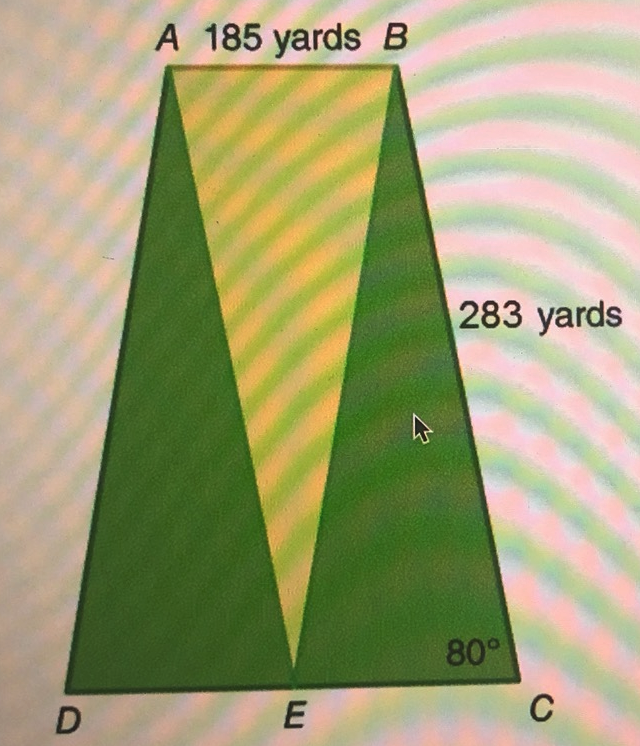
\includegraphics[width=0.90\columnwidth]{new_image}
    \caption{Land}
  \end{figure}
  Since the three isoceles triangles are congruent, we can define each isoceles triangle with the following dimensions:
\end{center}

\end{document}
